
\section{\label{alternative}Alternative definition for the social pressure}

Recall that the social force model (SFM) deals with the pedestrians desire and 
their private space preservation. Although the desire force 
$\mathbf{f}_d$ is a ``unilateral'' force, the Newton equations of 
motion remain valid. Therefore, it can be derived from the virial relation 
that \cite{lion}

\begin{equation}
 \bigg\langle\displaystyle\sum_{i=1}^N\displaystyle\frac{p_i^2}{m_i} + 
\displaystyle\sum_{i=1}^N 
\mathbf{r}_i\cdot\mathbf{f}_i\bigg\rangle=-2\mathcal{PA}\label{eqn_3}
\end{equation}


\noindent for the set of $N$ pedestrians inside an area $\mathcal{A}$. $p_i$  
and $\mathbf{f}_i$ are the momentum and total force acting on the individual 
$i$ 
(excluding the interaction with the walls). $\langle\cdot\rangle$ corresponds 
to 
the mean value along time. The right hand side $-2\mathcal{PA}$ defines the 
global pressure on the curve enclosing the surface $\mathcal{A}$.  \\

Following Ref.~\cite{lion} we can define the ``social pressure function'' $P_i$ 
as\\

\begin{equation}
2P_i\mathcal{A}_i=\displaystyle\frac{p_i^2}{m_i} + \frac{1}{2}
\displaystyle\sum_{j=1}^{N-1}
\mathbf{r}_{ij}\cdot\mathbf{f}_s^{(ij)}\label{eqn_4}
\end{equation}

\noindent where $\mathcal{A}_i$ is the area enclosing the pedestrian $i$ and 
$\mathbf{r}_{ij}=\mathbf{r}_{i}-\mathbf{r}_j$. Notice that the inner product 
$\mathbf{r}_{ij}\cdot\mathbf{f}_s^{(ij)}$ is always positive for repulsive 
feelings.  \\ 

The ``social pressure function'' $P_i$ is roughly similar to the literature 
definition \cite{Helbing1}, as expressed in Eq.~(\ref{eqn_4b}), for neglectable 
momentum $p_i$. Furthermore, Eqs.~(\ref{eqn_4b}) and (\ref{eqn_4}) become 
equal if the area $\mathcal{A}_i$ and $r_{ij}$ are replaced by $\pi r_i^2$ and 
the contacting distance $2r_i$, respectively. \\

We can further compute the pressure on all the pedestrians according to  
Eq.~(\ref{eqn_3}). Notice that the force sum can be split into the summation of 
three contributions:  the desire forces, the social forces and the granular 
forces. Actually, the granular force does not play a role because of 
orthogonality ($\mathbf{r}_{ij}\cdot\mathbf{f}_g^{(ij)}=0$). Consequently, 
replacing Eq.~(\ref{eqn_4}) into the virial relation (\ref{eqn_3}) gives \\  



\begin{equation}
 \displaystyle\sum_{i=1}^N\langle2P_i\mathcal{A}_i 
\rangle=-2\mathcal{PA}-\displaystyle\sum_{i=1}^N \langle
\mathbf{r}_i\cdot\mathbf{f}_d^{(i)}\rangle\label{eqn_5}
\end{equation}


We should remark that Eq.~(\ref{eqn_5}) holds either if the pedestrians are in 
contact or not. The ``social pressure function'' $P_i$ makes possible 
for the individuals to change their behavioural pattern when they come too 
close to each other. \\ 

\section{\label{app}The lane example}

We decided to open this supplementary section in order to make clear the 
meaning of the ``social pressure'' acting on an individual and the collective 
pressure (that is, the \textit{bulk} pressure) on a set of individuals. We 
will follow a simple example as a guide for more general situations. \\

\subsection{\label{social_pressure}The social pressure}

Fig.~\ref{fig:18} represents a lane of individuals pushing to the right. The 
ending wall prevents the individuals from moving. All the pedestrians in the 
lane are at their equilibrium positions $x_1,x_2,...,x_{i},...x_N$, 
while the wall is placed at the position $x_0=0$ (see Fig.~\ref{fig:18}).  \\

\begin{figure}[!htbp]
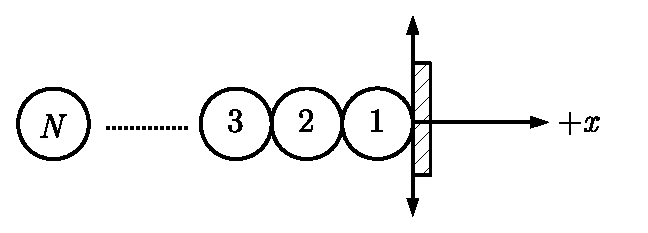
\includegraphics[width=0.75\columnwidth]{./fig15.eps}
\caption{\label{fig:18} Lane of individuals pushing to the right. The 
horizontal axis indicates the positive direction.  }
% done with figuras_presion.odg
\end{figure}

The pedestrians push to the right acknowledging a desired force 
$f_d^{(i)}=mv_d/\tau$, according to Eq.~(\ref{eqn_2}). The social repulsion 
feelings balance this desire force, but only the contacting neighbors are 
relevant to these feelings. Thus, the balance equation for any pedestrian 
in the lane reads \\

\begin{equation}
 f_s^{(i,i+1)}-f_s^{(i,i-1)}+\displaystyle\frac{mv_d}{\tau}=0\label{eqn_6}
\end{equation}

\noindent for $f_s^{(i,j)}$ meaning the repulsive feelings of pedestrian $i$ 
due to the presence of pedestrian $j$. Notice that the boundary condition at 
the wall-end is $x_0=0$ (Dirichlet condition), while the condition at the free 
end is $f_s^{(N,N+1)}=0$ (Neumann condition). The forces on the pedestrians can 
be obtained recursively from Eq.~\ref{eqn_6}, starting at the free ended 
individual ($i=N$). The resulting expression is 

\begin{equation}
f_s^{(i,i-1)}=(N-i+1)\,\displaystyle\frac{mv_d}{\tau}\ \ \ , \ \ \ 
i=1,....,N\label{eqn_7}
\end{equation}

\noindent while the corresponding positions $x_1,x_2,...,x_{i},...x_N$ are 
obtained by a backward substitution of the social forces expressed in 
Eq.~(\ref{eqn_2}), starting at the wall-end

\begin{equation} 
x_i=x_{i-1}-(r_{i}+r_{i-1})+B\,\ln\bigg[(N-i+1)\,\displaystyle\frac{mv_d}{A\tau}
\bigg]\label{eqn_8}
\end{equation}


The pressure on a single pedestrian $P_i$ corresponds to the forces acting on 
him (her) (per unit length) due to the neighboring pedestrians. According to 
Eqs.~(\ref{eqn_4b}), the pressure for any individual $i$ in the lane is  

\begin{equation}
P_i=\displaystyle\frac{1}{2\pi 
r_i}\,\bigg[f_s^ { (i , i+1) } +f_s^{(i,i-1)}\bigg]\label{eqn_10}
\end{equation}

We can also arrive to this expression through the ``social pressure 
function'' definition (\ref{eqn_4}) 

\begin{equation}
P_i=\displaystyle\frac{1}{2}\,\bigg[\displaystyle\frac{x_{i}-x_{i+1}}{
2\mathcal{A}_i } \,
f_s^ { (i , i+1) } +\displaystyle\frac { 
x_{i-1}-x_{i}}{2\mathcal{A}_i}\,f_s^{(i,i-1)}\bigg]\label{eqn_9}
\end{equation}

\vspace{3mm}

\noindent where the magnitude $x_{ij}/2\mathcal{A}_i$ corresponds to the 
(inverse) effective length of the pedestrian. For individuals modeled as 
circles, the inter-pedestrian distance is roughly $x_{ij}=2r_i$ and the area 
is $\mathcal{A}_i=\pi r_i^2$. Thus, both definitions agree. However, the 
last one is preferred since it does not assume that the forces actuate 
exactly at the distance $r_i$, as already mentioned in Section \ref{pressure}. 
\\


\subsection{\label{bulk_pressure}The bulk pressure}

We can now illustrate on how to compute the virial relation (\ref{eqn_5}). We 
can add the social pressures expressed in (\ref{eqn_9}) for the $N$
pedestrians in the lane.


\begin{equation}
\left\{\begin{array}{lcl}
2P_1\mathcal{A}_1 
& = &\displaystyle\frac{x_{1}}{2}f_s^ { (1 , 2)} - 
\displaystyle\frac{x_{2}}{2}\,f_s^ { (1 , 2) }  \\
&& \\
2P_2\mathcal{A}_2 
& = &\displaystyle\frac{x_{2}}{2}\,\big[f_s^ { (2 , 3)} - f_s^{(2,1)} 
\big] - \displaystyle\frac{x_{3}}{2}\,f_s^ { (2 , 3) } +\displaystyle\frac 
{ x_ {1}}{2}\,f_s^{(2,1) 
} \\
&& \\
2P_3\mathcal{A}_3 
& = &\displaystyle\frac{x_{3}}{2}\,\big[f_s^ { (3 , 4)} - f_s^{(3,2)} 
\big] - \displaystyle\frac{x_{4}}{2}\,f_s^ { (3 , 4) } +\displaystyle\frac 
{ x_{2}}{2}\,f_s^{(3,2) 
} \\
... &&\\
&& \\
2P_N\mathcal{A}_N 
& = &-\displaystyle\frac{x_{N}}{2}\, f_s^{(N,N-1)} 
+\displaystyle\frac{ x_{N-1}}{2}\,f_s^{(N,N-1) 
} \\
 \end{array}\right.\label{eqn_11}
\end{equation}

These are the local pressures on each pedestrian due to the 
contacting neighbors (and excluding the wall). Adding the terms results 
in the virial relation, as expressed in (\ref{eqn_5})

\begin{equation}
\begin{array}{lcl}
\displaystyle\sum_{i=1}^N 2P_i\mathcal{A}_i & = & (x_1 - x_2)f_s^{(1,2)} + (x_2 
- 
x_3)f_s^{(2,3)} +... \\
& + &  (x_{N-1}-x_N)f_s^{(N,N-1)} \\
&& \\
& = & x_{1}\,\displaystyle\frac{N\,mv_d}{\tau} - 
\displaystyle\sum_{i=1}^N x_i\,\displaystyle\frac{mv_d}{\tau} \\
 \end{array}\label{eqn_12}
\end{equation}

\noindent where the first term on the right corresponds to the global pressure 
$-2\mathcal{PA}$. Notice that $x_1$ is negative, and thus, $2\mathcal{PA}$ is 
defined as a positive magnitude. The last term is also positive, adding 
pressure to the bulk due to the desire forces.  
\\

The virial relation (\ref{eqn_5}) allows to compute the \textit{bulk} pressure 
on a group of pedestrians. For example, the pressure on the $M$ pedestrians 
closest to the wall corresponds to the force acting on this group due to the 
other $N-M$ pedestrians. According to Eq.~(\ref{eqn_5}), the 
pressure on the $M$ individuals is    


\begin{equation}
 \displaystyle\sum_{i=1}^M 2P_i\mathcal{A}_i 
=-2\mathcal{PA}-\displaystyle\sum_{i=M+1}^N 
2P_i\mathcal{A}_i-\displaystyle\sum_{i=1}^N 
x_i\displaystyle\frac{mv_d}{\tau}\label{eqn_13}
\end{equation}


The \textit{bulk} pressure on the first $M$ individuals increases as more 
individuals are included in the crowd. This can be verified by evaluating 
Eq.~(\ref{eqn_12}) and Eq.~(\ref{eqn_13}) for increasing values of $N$. \\

The Eqs.~(\ref{eqn_7}) and (\ref{eqn_8}) allow to compute the pedestrian 
pressure profile as a function of the distance to the wall. The profile is 
qualitatively similar to the one measured during an evacuation process. 
Fig.~\ref{fig:10} represents the histogram for the pressure on each 
pedestrian, computed as in Eq.~\ref{eqn_4b} and Eq.~\ref{eqn_4} (see caption for
details). \\


\begin{figure}[!htbp]
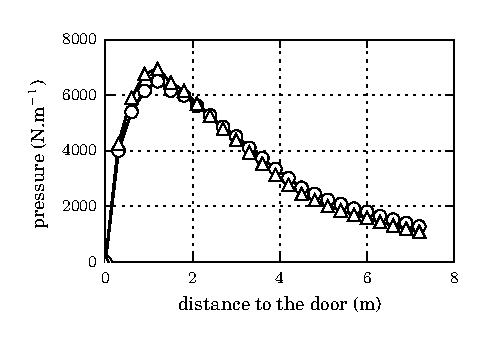
\includegraphics[width=\columnwidth]{./fig16.eps}
\caption{\label{fig:10} Mean pressure as a function of the distance 
to the exit. The room was $20\,\mathrm{m}\times20\,\mathrm{m}$ size and 
included one door of $d_w=1.2$~m width. Mean values were computed from 30 
evacuation processes, until 100 pedestrians left the room. The desired velocity 
was $v_d=4\,$m/s. The distance to the door was binned into equal intervals of 
$0.3$~m.  The $\bigcirc$  symbols correspond to the mean pressure computed as 
in \ref{eqn_4} for neglectable momentum ($p_i=0$) and $\mathcal{A}_i=\pi 
r_i^2$. The symbols $\bigtriangleup$ correspond to the mean pressure computed as 
in \ref{eqn_4b} (see text for details).  }
% done with fig10_version0.py 
\end{figure}

